\bookchapter{Cross-Compiling for ARM}\label{ch:rust10}

\section*{Explanation}
You write and test the program on a laptop, but it must run on the computer inside the robot, which has a \emph{different kind of processor}. A program compiled for one processor cannot run on another: the machine code is different, like a book in another language. \textbf{Cross-compiling} means to build, on the laptop, a program for the robot. This chapter explains the architecture names, shows the steps for the usual ARM robot computer, the typical problems (the C library, the linker, C dependencies), how to make the program small, how to copy it to the robot and swap it safely, and how to include the version in the program. We first look at real facts from a real machine, then at the steps.

\textbf{What was run.} The computer used to write this book is an x86-64 machine without access to \verb!crates.io! or to \verb!rustup!, and without an ARM cross-linker. Therefore the \emph{ARM-specific} commands (adding the target, linking, running with an emulator) were \textbf{not run}; the outputs that you see for them are marked ``expected''. What \emph{was} run: the compiler's own messages when the target is missing, the target lists, the size experiments, the version-embedding build script and the deployment script (in a local mode).

\section*{Which processor does your robot have?}
Ask the machine itself. On the robot (via SSH, Chapter~\ref{ch:linux3}):
\begin{verbatim}
$ uname -m
aarch64
\end{verbatim}
and on a laptop of the team this prints \verb!x86_64!. The main families:
\begin{center}
\renewcommand{\arraystretch}{1.2}
\begin{tabular}{lp{3.6cm}p{7cm}}
\textbf{\texttt{uname -m}} & \textbf{architecture} & \textbf{where}\\ \hline
\verb!x86_64! & Intel/AMD, 64 bit & laptops, desktops, many mini PCs\\
\verb!aarch64! & ARM, 64 bit (``ARM64'') & single-board computers, Jetson-class modules, phones, recent Macs\\
\verb!armv7l! & ARM, 32 bit & older small boards\\
\end{tabular}
\end{center}
Check the manual of \emph{your} robot for the computer that it has; do not assume. (This book does not give hardware data for a specific robot that it cannot verify.) The robot computer is usually ARM because ARM processors give a lot of computing power for little electrical power (Chapter~\ref{ch:hw8}).

\section*{The target triple}
Rust names a platform with a \textbf{target triple}: architecture, vendor, operating system and (often) the C library, joined by hyphens.
\begin{center}
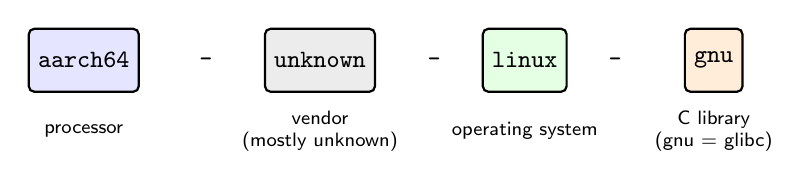
\begin{tikzpicture}[font=\ttfamily\small]
 \node[draw,thick,rounded corners=2pt,fill=blue!10,minimum height=0.8cm] (a) at (0,0) {aarch64};
 \node at (1.55,0) {-};
 \node[draw,thick,rounded corners=2pt,fill=gray!15,minimum height=0.8cm] (v) at (3.0,0) {unknown};
 \node at (4.45,0) {-};
 \node[draw,thick,rounded corners=2pt,fill=green!10,minimum height=0.8cm] (o) at (5.6,0) {linux};
 \node at (6.75,0) {-};
 \node[draw,thick,rounded corners=2pt,fill=orange!15,minimum height=0.8cm] (e) at (8.0,0) {gnu};
 \node[font=\sffamily\scriptsize,align=center] at (0,-0.9) {processor};
 \node[font=\sffamily\scriptsize,align=center] at (3.0,-0.9) {vendor\\ (mostly unknown)};
 \node[font=\sffamily\scriptsize,align=center] at (5.6,-0.9) {operating system};
 \node[font=\sffamily\scriptsize,align=center] at (8.0,-0.9) {C library\\ (gnu = glibc)};
\end{tikzpicture}
\captionof{figure}{The target triple of a 64-bit ARM Linux system with the usual GNU C library.}
\end{center}
The compiler knows many of them (\verb!rustc --print target-list!). The relevant ones for robots:
\begin{center}
\renewcommand{\arraystretch}{1.2}
\begin{tabular}{lp{7.2cm}}
\verb!x86_64-unknown-linux-gnu! & your laptop (the \emph{host})\\
\verb!aarch64-unknown-linux-gnu! & a 64-bit ARM Linux robot computer with Ubuntu or Debian\\
\verb!aarch64-unknown-linux-musl! & the same processor, statically linked with the small musl C library\\
\verb!armv7-unknown-linux-gnueabihf! & 32-bit ARM Linux with hardware floating point\\
\end{tabular}
\end{center}
The compiler can print what it knows about a target, for example (the real output):
\begin{verbatim}
$ rustc --print cfg --target aarch64-unknown-linux-gnu | grep target_
target_arch="aarch64"
target_endian="little"
target_env="gnu"
target_os="linux"
target_pointer_width="64"
\end{verbatim}
These are the values that you test in a program with \verb!#[cfg(target_arch = "aarch64")]! if some code must differ between machines.

\section*{What is needed to build for another processor}
\begin{center}
\begin{tikzpicture}[>={Stealth[length=2.4mm]},bx/.style={draw,thick,rounded corners=2pt,minimum width=3.0cm,minimum height=1.0cm,font=\footnotesize,align=center}]
 \node[bx,fill=blue!10] (src) at (0,0) {your source\\ (\texttt{.rs} files)};
 \node[bx,fill=yellow!20] (rc) at (4.2,0) {\texttt{rustc}\\ + standard library\\ \emph{for the target}};
 \node[bx,fill=orange!15] (ld) at (8.4,0) {linker\\ \emph{for the target}\\ + C library files};
 \node[bx,fill=green!10] (bin) at (12.6,0) {ARM executable};
 \draw[->,thick] (src)--(rc); \draw[->,thick] (rc)--node[above,font=\scriptsize]{object files} (ld); \draw[->,thick] (ld)--(bin);
 \node[font=\scriptsize,gray,align=center] at (4.2,-1.1) {\texttt{rustup target add ...}};
 \node[font=\scriptsize,gray,align=center] at (8.4,-1.1) {\texttt{apt install gcc-aarch64-linux-gnu}};
\end{tikzpicture}
\captionof{figure}{Rust's compiler is a cross-compiler already; what you must add is the standard library of the target and a linker that can produce code for the target.}
\end{center}
\textbf{The compiler} of Rust (built on LLVM) can generate code for many processors, but needs the \textbf{standard library} compiled for the target. You install it with rustup. If you forget, the compiler says so (the real message, from this computer, which has no ARM target):
\begin{verbatim}
$ cargo build --target aarch64-unknown-linux-gnu
   Compiling hello v0.1.0 (/home/student/hello)
error[E0463]: can't find crate for `std`
  |
  = note: the `aarch64-unknown-linux-gnu` target may not be installed
  = help: consider downloading the target with
          `rustup target add aarch64-unknown-linux-gnu`
\end{verbatim}
\textbf{The linker} joins the object files with the parts of the C library. The linker of your laptop only knows x86. On Ubuntu a cross-linker for ARM comes as a package.

\section*{Step by step: Ubuntu laptop to ARM64 robot}
\textbf{Not run} on the computer of the book (no network, no ARM linker); this is the standard procedure.
\begin{verbatim}
$ rustup target add aarch64-unknown-linux-gnu
$ sudo apt install gcc-aarch64-linux-gnu
\end{verbatim}
Tell cargo which linker to use for this target, in the file \verb!.cargo/config.toml! inside the project (or in \verb!~/.cargo/config.toml! for all projects):
\begin{verbatim}
[target.aarch64-unknown-linux-gnu]
linker = "aarch64-linux-gnu-gcc"
\end{verbatim}
Build and check:
\begin{verbatim}
$ cargo build --release --target aarch64-unknown-linux-gnu
$ file target/aarch64-unknown-linux-gnu/release/robot-app
... ELF 64-bit LSB pie executable, ARM aarch64, version 1 (SYSV),
    dynamically linked, interpreter /lib/ld-linux-aarch64.so.1, ...
\end{verbatim}
(The \verb!file! line is the \emph{expected} output.) The result lands in a separate folder, \verb!target/<triple>/release/!. For comparison, the real output of \verb!file! for a program built on this computer for itself:
\begin{verbatim}
$ file target/release/hello
target/release/hello: ELF 64-bit LSB pie executable, x86-64, version 1
(SYSV), dynamically linked, interpreter /lib64/ld-linux-x86-64.so.2,
for GNU/Linux 3.2.0, ...
\end{verbatim}
The words after the comma name the architecture: that is how you check that a file is for the machine it is meant for. If you start an ARM program on the laptop (or the other way round) the shell answers \verb!cannot execute binary file: Exec format error!: the processor cannot understand the file.

Rust programs that use only the standard library, as in this book, cross-compile without further work. The sections below deal with what goes wrong in bigger programs.

\subsection*{Problem 1: the C library version}
A program built with the \verb!gnu! target is \emph{dynamically linked}: it uses the C library \verb!libc.so! of the computer where it runs, and records the \emph{oldest version} of this library that it needs. A program built on a newer system needs a newer library than an older robot system has. The needed versions can be read from the file (real output for a hello program built on Ubuntu~24.04 with glibc~2.39):
\begin{verbatim}
$ objdump -T target/release/hello | grep -o "GLIBC_[0-9.]*" \
    | sort -uV | tail -2
GLIBC_2.33
GLIBC_2.34
\end{verbatim}
On a system whose glibc is older than $2.34$ this program does not start: \verb!version `GLIBC_2.34' not found!. Remedies:
\begin{itemize}[nosep]
\item Build on (or in a container of) the \emph{oldest} system that you must support, or use the \emph{same} Ubuntu release on laptop and robot. The team's laptops and robots should run the same release; that avoids the problem (Chapter~\ref{ch:linux4}).
\item Link \textbf{statically} against musl with the target \verb!aarch64-unknown-linux-musl!: the executable contains its C library and runs on any 64-bit ARM Linux. Costs: some crates with C dependencies do not build, and the memory allocator of musl is slower than the one of glibc (in multi-threaded programs the difference can be large; measure it).
\item Cross-compile with \verb!cross! or \verb!cargo-zigbuild! (below), which can target an old glibc version.
\end{itemize}

\subsection*{Problem 2: C dependencies}
A pure Rust crate cross-compiles without effort. A crate that wraps a C library (OpenSSL, a camera driver, \verb!libudev!, a serial port library) needs the \emph{ARM version of that C library} and its header files, and the build script must find them (via \verb!pkg-config!, with the environment variable \verb!PKG_CONFIG_SYSROOT_DIR!). This is the main source of pain. Strategies: prefer \textbf{pure Rust crates} (for example \verb!rustls! instead of OpenSSL); use crate features that \emph{vendor} the C code and build it with the cross-compiler (many crates have a feature called \verb!vendored! or \verb!bundled!); or build in a container that has the ARM libraries (the next section). Note that build scripts (\verb!build.rs!, like the \verb!prost-build! script of Chapter~\ref{ch:rust8}) run on the \emph{host}, not on the target; \verb!protoc! is therefore installed on the laptop, not on the robot.

\section*{Easier tools}
\begin{center}
\renewcommand{\arraystretch}{1.2}
\begin{tabular}{lp{9.4cm}}
\verb!cross! & wraps cargo: \verb!cross build --target aarch64-unknown-linux-gnu! runs the build in a Docker or Podman container that contains the cross-compiler and libraries; works out of the box for most cases and can also \emph{run} tests under an emulator. Needs a container engine.\\
\verb!cargo-zigbuild! & uses the C compiler of the Zig project as linker and can select the glibc version: \verb!--target aarch64-unknown-linux-gnu.2.31! builds for glibc $2.31$.\\
native build on ARM & build \emph{on} the robot, or on an ARM server in CI (GitHub offers ARM runners): no cross-compilation problems at all; slower, and needs a toolchain on the machine. For a big project the first full build can take many minutes.\\
\end{tabular}
\end{center}
These tools were not run for the book; read their documentation for the current options.

\section*{Testing without the robot}
The emulator \textbf{QEMU} can run an ARM program on an x86 laptop (``user mode'' translates the instructions, the system calls are passed to the host):
\begin{verbatim}
$ sudo apt install qemu-user gcc-aarch64-linux-gnu
$ qemu-aarch64 -L /usr/aarch64-linux-gnu \
    target/aarch64-unknown-linux-gnu/release/robot-app
\end{verbatim}
The option \verb!-L! tells QEMU where to find the ARM C library. Cargo can use it for the tests as well, with one more entry in \verb!.cargo/config.toml!:
\begin{verbatim}
[target.aarch64-unknown-linux-gnu]
linker = "aarch64-linux-gnu-gcc"
runner = "qemu-aarch64 -L /usr/aarch64-linux-gnu"
\end{verbatim}
and then \verb!cargo test --target aarch64-unknown-linux-gnu! runs the unit tests of the ARM build on the laptop. This finds errors that depend on the architecture (size of types, alignment, byte order); QEMU is slow and does not reproduce timing, so measurements must be made on the real robot. (Not run for the book.)

\section*{Making the program small and fast}
The release profile in \verb!Cargo.toml! controls the build. We measured the effect of the options on a small program (a \verb!HashMap! and the arguments; size of the executable in bytes, on this computer):
\begin{center}
\renewcommand{\arraystretch}{1.2}
\begin{tabular}{lr}
\textbf{setting in \texttt{[profile.release]}} & \textbf{size}\\ \hline
default & 465\,864\\
\verb!strip = true! & 357\,864\\
\verb!+ lto = true, codegen-units = 1, panic = "abort"! & 320\,976\\
\verb!+ opt-level = "z"! & 302\,360\\
\end{tabular}
\end{center}
\begin{itemize}[nosep]
\item \verb!strip = true! removes the symbol names and debugging information, which are only needed for crash analysis: $23\,\%$ smaller here. Keep an unstripped copy of each release that you put on a robot, so that a crash can still be understood.
\item \verb!lto = true! (link time optimisation) lets the compiler optimise \emph{across} crates, \verb!codegen-units = 1! gives it the whole crate at once: smaller and often faster code, but a much slower build; use it for the release that goes to the robot, not for every test build.
\item \verb!panic = "abort"! ends the program immediately on a panic instead of unwinding the stack (Chapter~\ref{ch:rust5}): smaller and faster, but no \verb!catch_unwind! and no clean-up. A robot program that cannot continue after a panic is better aborted, and a supervisor (systemd, below) restarts it.
\item \verb!opt-level = "z"! optimises for size, \verb!"s"! similar, \verb!3! (the default) for speed. Never use \verb!"z"! for a real-time loop without measuring.
\end{itemize}
The program here is tiny, so the percentages are not typical for a larger one; the \emph{method} is: change one setting, build, measure the size and, more importantly, the speed (Chapter~\ref{ch:ai9}). And do not use \verb!-C target-cpu=native! in a cross-build: it optimises for the processor of the \emph{laptop}, and the program can crash with ``illegal instruction'' on the robot.

\section*{Which version is running?}
A bug report that says ``the robot did something strange'' is useless if nobody knows which program was running. Put the version and the commit into the program. The version is available to every crate as \verb|env!("CARGO_PKG_VERSION")|. The commit hash can be added by a build script. We ran the following (the build script runs on the host):
\begin{verbatim}
// build.rs
use std::process::Command;

fn main() {
    let hash = Command::new("git")
        .args(["rev-parse", "--short", "HEAD"])
        .output()
        .ok()
        .filter(|o| o.status.success())
        .map(|o| String::from_utf8_lossy(&o.stdout).trim().to_string())
        .unwrap_or_else(|| "unknown".to_string());
    println!("cargo:rustc-env=GIT_HASH={hash}");
    println!("cargo:rerun-if-changed=.git/HEAD");
}
\end{verbatim}
\begin{verbatim}
// src/main.rs
fn main() {
    println!(
        "robot-app {} ({}) built for {}",
        env!("CARGO_PKG_VERSION"),
        env!("GIT_HASH"),
        std::env::consts::ARCH,
    );
}
\end{verbatim}
Outside a git repository the output was \verb!robot-app 0.1.0 (unknown) built for x86_64!, after \verb!git init! and a commit \verb!robot-app 0.1.0 (d769451) built for x86_64!. On the robot, the same program built for ARM prints \verb!aarch64! at the end. Print this line at the start of every run and write it into the log.

\section*{Getting the program onto the robot}
Copy the file with \verb!scp! or \verb!rsync! (Chapter~\ref{ch:linux3}) and start it. Three rules for a deployment that does not break the robot: never overwrite a running program in place (the file is busy, and a half-copied file is a broken program); keep the \emph{previous version} so that you can go back in seconds; verify that what arrived is what you sent. The following script does all three: it uploads under a new name, verifies the checksum, and then replaces the old file with one \verb!mv!, which is atomic. It was tested in its local mode (without a host the files are copied into a local folder); with a host the commands go through \verb!ssh! and \verb!scp!.
\begin{verbatim}
#!/usr/bin/env bash
# usage: deploy.sh <binary> [user@host]    (no host: copy locally)
set -euo pipefail

BIN=${1:?usage: deploy.sh <binary> [user@host]}
HOST=${2:-}
DIR=${DEPLOY_DIR:-/opt/robot}

sum=$(sha256sum "$BIN" | cut -d' ' -f1)
echo "deploying $(basename "$BIN") sha256=${sum:0:12}"

run()  { if [ -n "$HOST" ]; then ssh "$HOST" "$@"; else bash -c "$*"; fi; }
send() {
    if [ -n "$HOST" ]; then scp -q "$1" "$HOST:$2"; else cp "$1" "$2"; fi
}

run "mkdir -p $DIR"
# 1. upload next to the old file
send "$BIN" "$DIR/robot-app.new"
# 2. verify the checksum on the robot
run "cd $DIR && echo '$sum  robot-app.new' | sha256sum -c --quiet"
# 3. keep the old file, swap in the new one (mv is atomic)
run "cd $DIR && chmod +x robot-app.new \
     && { [ -f robot-app ] && mv -f robot-app robot-app.prev || true; } \
     && mv robot-app.new robot-app"
echo "done; roll back with: mv -f $DIR/robot-app.prev $DIR/robot-app"
\end{verbatim}
(\verb!set -euo pipefail! makes the script stop at the first error, Chapter~\ref{ch:linux2}.) Running it twice in the local test left the folder with \verb!robot-app! and \verb!robot-app.prev!, and the new \verb!robot-app! started and printed its version. The program is then started by \textbf{systemd} (Chapter~\ref{ch:linux5}), which restarts it when it ends abnormally and starts it at boot:
\begin{verbatim}
[Unit]
Description=Robot application
After=network-online.target
Wants=network-online.target

[Service]
ExecStart=/opt/robot/robot-app
Restart=on-failure
RestartSec=1
User=robot
Environment=RUST_BACKTRACE=1

[Install]
WantedBy=multi-user.target
\end{verbatim}
saved as \verb!/etc/systemd/system/robot-app.service!; then \verb!sudo systemctl enable --now robot-app! and \verb!journalctl -u robot-app -f! for the log. (The syntax of this unit file was checked with \verb!systemd-analyze verify!; the only complaint was that the program does not exist on the book computer.) For a competition, a one-line build-and-deploy command (a \verb!justfile!, a \verb!Makefile!, or a ten-line script) is worth much more than a perfect procedure that nobody remembers under stress.

\begin{aibox}[The release checklist]
(1) The tests pass on the laptop. (2) Build for the target with the release profile. (3) \verb!file! says the right architecture. (4) The program prints its version and commit. (5) Upload under a new name, verify the checksum, keep the previous version. (6) Start it on the robot \emph{in a safe state} (robot on a stand, Chapter~\ref{ch:hw8}) and watch the first minutes of the log. (7) Tag the commit in git (Chapter~\ref{ch:git3}) so that you can always rebuild exactly this program.
\end{aibox}

\section*{Practice problems}
\begin{enumerate}[label=\textbf{\thechapter.\arabic*}]
  \item Which command tells you the architecture of the robot computer? Which command tells you the architecture of an executable file?
  \item Explain the parts of the target triple \verb!aarch64-unknown-linux-gnu!. What changes if you replace \verb!gnu! by \verb!musl!?
  \item The command \verb!cargo build --target aarch64-unknown-linux-gnu! says ``can't find crate for `std'\,''. What is missing and how do you add it? After that the error is \verb!linker `cc' not found! or the linker complains about the wrong architecture. What do you do?
  \item Write the contents of \verb!.cargo/config.toml! for cross-compiling to \verb!aarch64-unknown-linux-gnu! with the linker \verb!aarch64-linux-gnu-gcc! and QEMU as test runner.
  \item On the robot your program ends with \verb!version `GLIBC_2.38' not found!. Explain what happened and name two ways to fix it.
  \item You get \verb!cannot execute binary file: Exec format error! on the robot. Which two mistakes could be the cause, and how do you decide with one command?
  \item A project uses a crate that needs OpenSSL. Give three ways to get it to cross-compile. Which would you try first and why?
  \item A release binary has $12.4$\,MB. List four measures to reduce the size and say what each one costs.
  \item Why do you keep an unstripped copy of every deployed binary? Where do you store it?
  \item[\textbf{\thechapter.10}$\star$] Write the \verb!justfile! or the \verb!Makefile! (your choice) with the targets \verb!test!, \verb!build-arm!, \verb!deploy! and \verb!logs! so that \verb!just deploy ROBOT=robot3.local! (or \verb!make deploy ROBOT=...!) runs the tests, builds the ARM release, checks with \verb!file! that the architecture is right, calls the deployment script and restarts the service. Which of the steps should stop the whole process when it fails?
\end{enumerate}
